\documentclass[12pt,letterpaper]{article}
\usepackage{graphicx,textcomp}
\usepackage{natbib}
\usepackage{setspace}
\usepackage{fullpage}
\usepackage{color}
\usepackage[reqno]{amsmath}
\usepackage{amsthm}
\usepackage{fancyvrb}
\usepackage{amssymb,enumerate}
\usepackage[all]{xy}
\usepackage{endnotes}
\usepackage{lscape}
\newtheorem{com}{Comment}
\usepackage{float}
\usepackage{hyperref}
\newtheorem{lem} {Lemma}
\newtheorem{prop}{Proposition}
\newtheorem{thm}{Theorem}
\newtheorem{defn}{Definition}
\newtheorem{cor}{Corollary}
\newtheorem{obs}{Observation}
\usepackage[compact]{titlesec}
\usepackage{dcolumn}
\usepackage{tikz}
\usetikzlibrary{arrows}
\usepackage{multirow}
\usepackage{xcolor}
\newcolumntype{.}{D{.}{.}{-1}}
\newcolumntype{d}[1]{D{.}{.}{#1}}
\definecolor{light-gray}{gray}{0.65}
\usepackage{url}
\usepackage{listings}
\usepackage{color}

\definecolor{codegreen}{rgb}{0,0.6,0}
\definecolor{codegray}{rgb}{0.5,0.5,0.5}
\definecolor{codepurple}{rgb}{0.58,0,0.82}
\definecolor{backcolour}{rgb}{0.95,0.95,0.92}

\lstdefinestyle{mystyle}{
	backgroundcolor=\color{backcolour},   
	commentstyle=\color{codegreen},
	keywordstyle=\color{magenta},
	numberstyle=\tiny\color{codegray},
	stringstyle=\color{codepurple},
	basicstyle=\footnotesize,
	breakatwhitespace=false,         
	breaklines=true,                 
	captionpos=b,                    
	keepspaces=true,                 
	numbers=left,                    
	numbersep=5pt,                  
	showspaces=false,                
	showstringspaces=false,
	showtabs=false,                  
	tabsize=2
}
\lstset{style=mystyle}
\newcommand{\Sref}[1]{Section~\ref{#1}}
\newtheorem{hyp}{Hypothesis}

\title{Problem Set 3}
\date{Due: November 12, 2026}
\author{Applied Stats/Quant Methods 1}


\begin{document}
	\maketitle
	\section*{Instructions}
	\begin{itemize}
		\item Please show your work! You may lose points by simply writing in the answer. If the problem requires you to execute commands in \texttt{R}, please include the code you used to get your answers. Please also include the \texttt{.R} file that contains your code. If you are not sure if work needs to be shown for a particular problem, please ask.
	\item Your homework should be submitted electronically on GitHub.
	\item This problem set is due before 23:59 on Thursday November 12, 2026. No late assignments will be accepted.

	\end{itemize}

		\vspace{.25cm}
	
\noindent In this problem set, you will run several regressions and create an add variable plot (see the lecture slides) in \texttt{R} using the \texttt{incumbents\_subset.csv} dataset. Include all of your code.

	\vspace{.5cm}
\section*{Question 1}
\vspace{.25cm}
\noindent We are interested in knowing how the difference in campaign spending between incumbent and challenger affects the incumbent's vote share. 
	\begin{enumerate}
		\item Run a regression where the outcome variable is \texttt{voteshare} and the explanatory variable is \texttt{difflog}. \vspace{0.5cm}
				
		\lstinputlisting[firstline = 43, lastline = 44]{PS03_AL.R}
		
		Looking at (the Coefficents part of) the output from the second line, we can obtain all relevant information for interpreting our regression estimate.
		
		\begin{verbatim}
		Coefficients:
		Estimate Std. Error t value Pr(>|t|)    
		(Intercept) 0.579031   0.002251  257.19   <2e-16 ***
		difflog     0.041666   0.000968   43.04   <2e-16 ***			
		\end{verbatim}
		
		The intercept has a value of 0.579; accordingly, candidates on average receive 57.9 percent of the votes if the independent variable \texttt{difflog} equals zero. The estimate is statistically reliable; however, the significance of the intercept is commonly not informative. 
		The estimated slope for difflog is 0.041. On average, the candidates vote share increases by 4.1 percent for every additional unit of difflog. The effect is statistically reliable, as $|t| > 1{,}96$, and $p < 0{,}05$.
		
		\vspace{1cm}
		\item Make a scatterplot of the two variables and add the regression line. 	
		
		I used the following R code to create the scatterplot
		\lstinputlisting[firstline = 48, lastline = 59]{PS03_AL.R}
		
		\begin{figure}[h!]\centering
			\caption{\footnotesize Campaign Spending and Vote Share.}
			\label{fig:plot_1}
			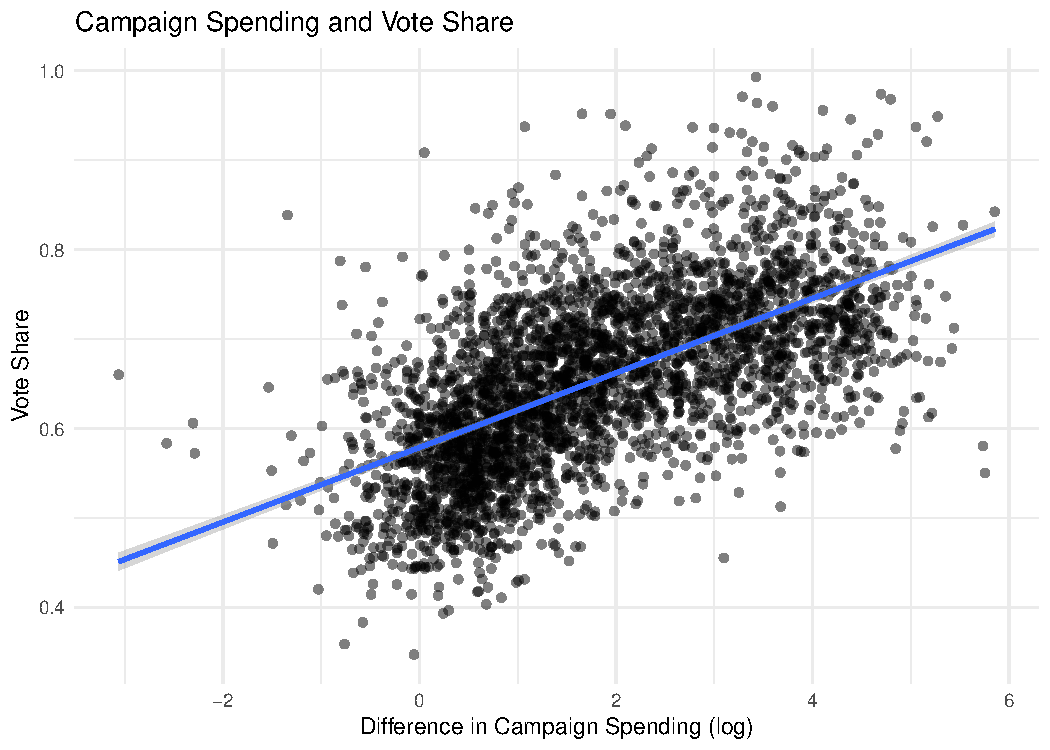
\includegraphics[width=.75\textwidth]{plot1.pdf}
		\end{figure}
		
		\newpage
		
		
		\item Save the residuals of the model in a separate object.	\vspace{1cm}
		
		We can extract the residuals from the \textbf{lm object model1}.
		
		\lstinputlisting[firstline = 68, lastline = 68]{PS03_AL.R}
		
		\vspace{2cm}
		\item Write the prediction equation.
		
		Using the general equation for linear regression we get. 
		\[\widehat{\text{Voteshare}} = \alpha + \beta_1 \cdot \text{difflog}\]
		Putting in concrete values from our regress model we get \[\widehat{\text{Voteshare}} = 0.579 + \text{0.041} \cdot \text{difflog} \]
		
	\end{enumerate}
	
\newpage

\section*{Question 2}
\noindent We are interested in knowing how the difference between incumbent and challenger's spending and the vote share of the presidential candidate of the incumbent's party are related.	\vspace{.25cm}
	\begin{enumerate}
		\item Run a regression where the outcome variable is \texttt{presvote} and the explanatory variable is \texttt{difflog}.	\vspace{0.5cm}
		
		\lstinputlisting[firstline = 43, lastline = 44]{PS03_AL.R}
		Looking at (the Coefficents part of) the output from the second line, we can obtain all relevant information for interpreting our regression estimate.
		
		\begin{verbatim}
		Coefficients:
		Estimate Std. Error t value Pr(>|t|)    
		(Intercept) 0.507583   0.003161  160.60   <2e-16 ***
		difflog     0.023837   0.001359   17.54   <2e-16 ***			
		\end{verbatim}
		
		The intercept is rounded to 0.508; accordingly, the presidential candidate of the incumbent's party on average receives approximately 50.8 percent of the votes when the independent variable \texttt{difflog} equals zero. The estimate is statistically reliable; however, the intercept is often not informative. 
		The estimated slope for difflog is 0.0231. On average, the incumbent party presidential candidate's vote share increases by 2.3 percent for every additional unit of difflog. The effect is statistically reliable, as $|t| > 1{,}96$, and $p < 0{,}05$.
		\vspace*{0.5cm}
		\item Make a scatterplot of the two variables and add the regression line. 
		
		I used the following R code to create the scatterplot
		\lstinputlisting[firstline = 89, lastline = 97]{PS03_AL.R}
		
		\begin{figure}[h!]\centering
			\caption{\footnotesize Campaign Spending and Presidental Candidates Success.}
			\label{fig:plot_2}
			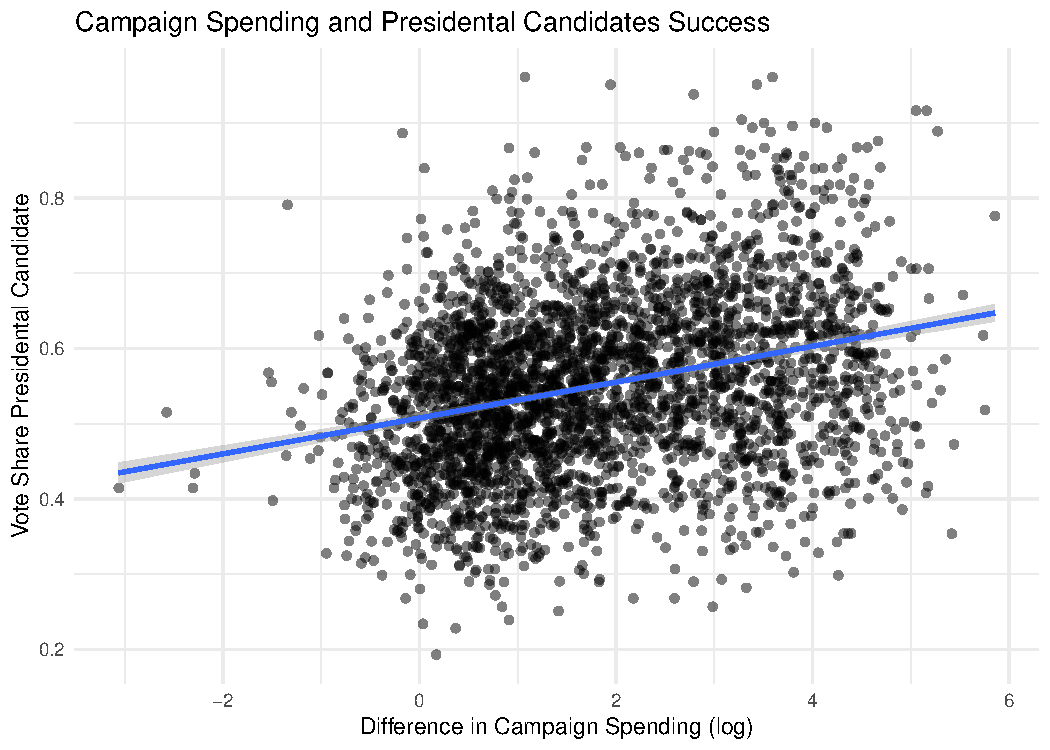
\includegraphics[width=.75\textwidth]{plot2.pdf}
		\end{figure}
		
		\vspace{1.5cm}
				
		\item Save the residuals of the model in a separate object.	
		We can extract the residuals from the \textbf{lm object model2}.
		\lstinputlisting[firstline = 108, lastline = 108]{PS03_AL.R}
		\vspace{1cm}
		\item Write the prediction equation.
		
		Using the general equation for linear regression we get. 
		\[\widehat{\text{Inc. Party Presidental Candidate}} = \alpha + \beta_1 \cdot \text{difflog}\]
		Putting in concrete values from our regress model we get \[\widehat{\text{Inc. Party Presidental Candidate}} = 0.508 + \text{0.023} \cdot \text{difflog}\]
	
		
	\end{enumerate}
	
	\newpage	
\section*{Question 3}

\noindent We are interested in knowing how the vote share of the presidential candidate of the incumbent's party is associated with the incumbent's electoral success.
	\vspace{.25cm}
	\begin{enumerate}
		\item Run a regression where the outcome variable is \texttt{voteshare} and the explanatory variable is \texttt{presvote}.
			
		\lstinputlisting[firstline = 120, lastline = 121]{PS03_AL.R}
		Looking at (the Coefficents part of) the output from the second line, we can obtain all relevant information for interpreting our regression estimate.
		
		\begin{verbatim}
		Coefficients:
		Estimate Std. Error t value Pr(>|t|)    
		(Intercept) 0.441330   0.007599   58.08   <2e-16 ***
		presvote    0.388018   0.013493   28.76   <2e-16 ***		
		\end{verbatim}
		
		The intercept is rounded to 0.441; accordingly, the vote share of candidates is 44.1 on average if the incumbent party's presidential candidate has a vote share of 0 per cent. This scenario is very unrealistic, and therefore not very informative.  
		The estimated slope for difflog is 0.388. On average, vote share increases by 38.8 percent for every additional unit in the incumbent party presidential candidate's vote share. However, this explanatory variable is measured as a fraction with a range between 0 and 1; accordingly, the 38.8 percent change occurs if an incumbent party presidential candidate gains an additional 100 percent in vote share. We should consider transforming the variable to recalculate the model.
		The effect is statistically reliable, as $|t| > 1{,}96$, and $p < 0{,}05$.
			
						
		\item Make a scatterplot of the two variables and add the regression line. 
		
		I used the following R code to create the scatterplot
		\lstinputlisting[firstline = 124, lastline = 135]{PS03_AL.R}
		
		\begin{figure}[h!]\centering
			\caption{\footnotesize  Presidental Candidates Success and Vote Shares.}
			\label{fig:plot_3}
			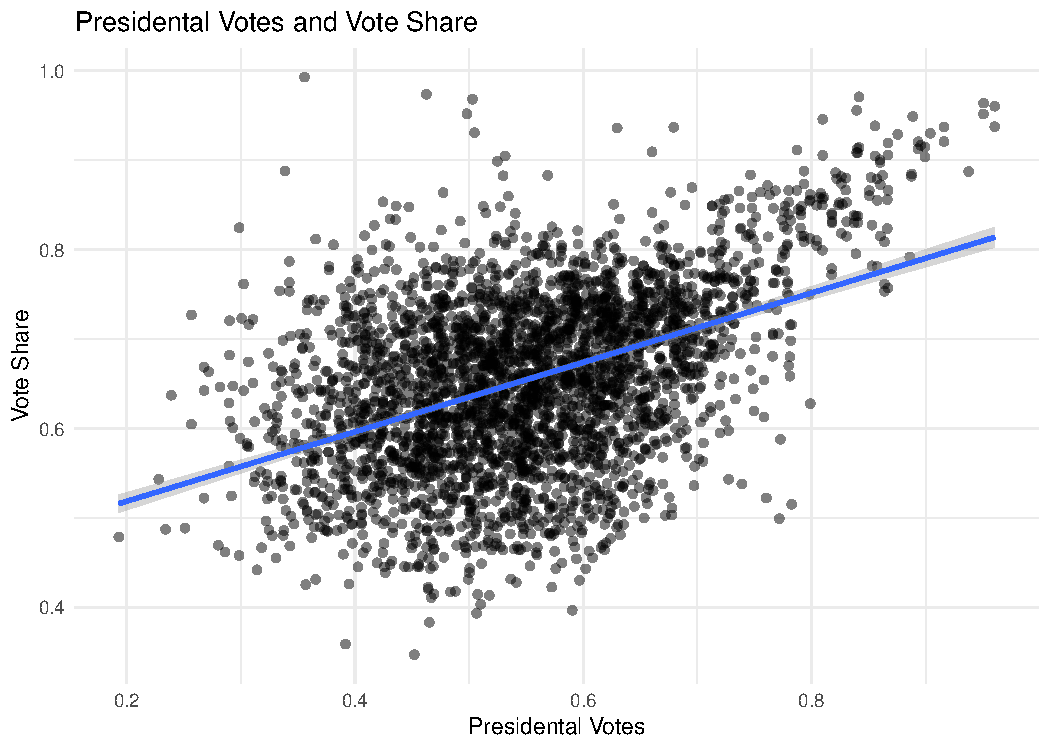
\includegraphics[width=.75\textwidth]{plot3.pdf}
		\end{figure}
			
		\newpage
		\item Write the prediction equation.
		Using the general equation for linear regression we get.
		\[\widehat{\text{Vote Share}} = \alpha + \beta_1 \cdot \text{Inc. Party Presidental Candidate}\]
		Putting in concrete values from our regress model we get \[\widehat{\text{Vote Share}} = 0.441 + \text{Inc. Party Presidental Candidate} \cdot \text{0.388} \]
				
	\end{enumerate}
	

\newpage	
\section*{Question 4}
\noindent The residuals from part (a) tell us how much of the variation in \texttt{voteshare} is $not$ explained by the difference in spending between incumbent and challenger. The residuals in part (b) tell us how much of the variation in \texttt{presvote} is $not$ explained by the difference in spending between incumbent and challenger in the district.
	\begin{enumerate}
		\item Run a regression where the outcome variable is the residuals from Question 1 and the explanatory variable is the residuals from Question 2.	\vspace{0.5cm}
				
		I begin by combining the two vectors from the previous task into a common dataset. Then I estimate the regression model. 
		\lstinputlisting[firstline = 158, lastline = 160]{PS03_AL.R}
		
		Looking at (the Coefficents part of) the output from the second line, we can obtain all relevant information for interpreting our regression estimate.
		
		\begin{verbatim}
		Coefficients:
		Estimate Std. Error t value Pr(>|t|)    
		(Intercept)   -5.934e-18  1.299e-03    0.00        1    
		errors_model2  2.569e-01  1.176e-02   21.84   <2e-16 ***		
		\end{verbatim}
		
		The intercept is virtually 0. On average, an observation with no unexplained variance in model2 also has no unexplained variance in model 1. Substantively, this means that cases that are well explained by differences in campaign spending in one model are also close to the estimates in the other model, which seems reasonable since the same explanatory variable was used to explain similar concepts.
		The slope is approximately 0.257. On average, for every unit increase in the residuals from model 2, the residuals from model 1 increase by 0.257 units. Substantively, the residuals of model 2 measure the part of incumbents' party presidential vote share that is not explained by campaign spending, while the residuals from model 1 measure the variance of vote share that is not explained by campaign spending (see Question 5).
		
		
		\item Make a scatterplot of the two residuals and add the regression line. 	
		
		I used the following R code to create the scatterplot
		\lstinputlisting[firstline = 163, lastline = 172]{PS03_AL.R}
		
		\begin{figure}[h!]\centering
			\caption{\footnotesize  Scatterplot of the Residuals.}
			\label{fig:plot_4}
			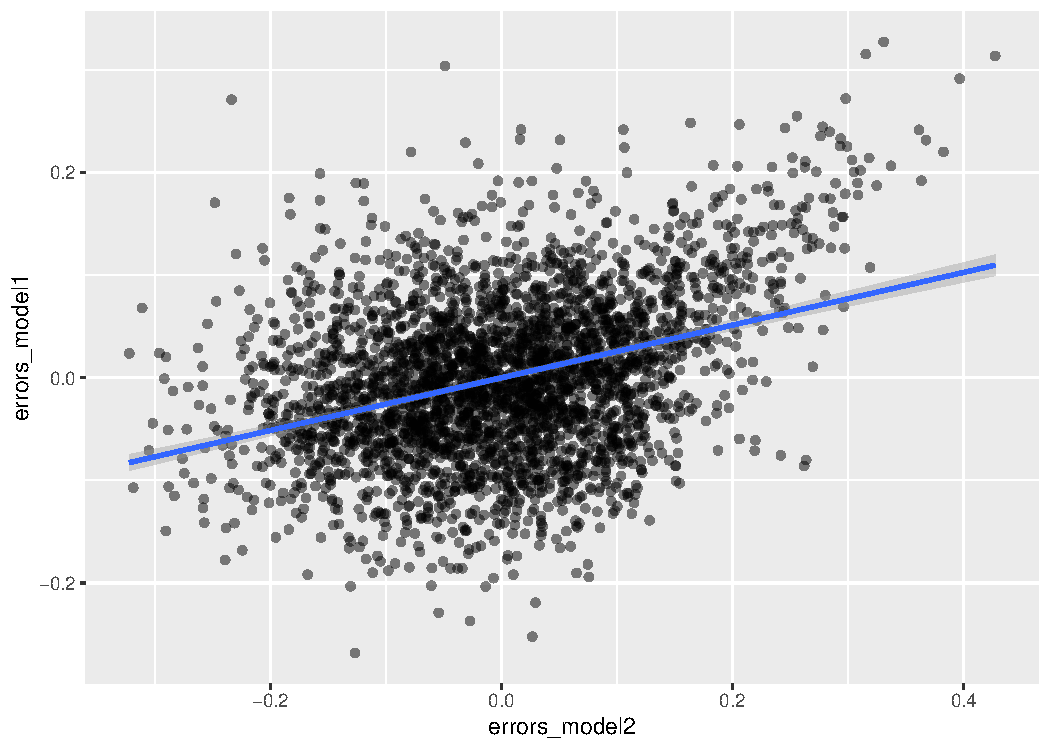
\includegraphics[width=.75\textwidth]{plot4.pdf}
		\end{figure}
		
	\item Write the prediction equation.
	
	Using the general equation for linear regression, we get:
	\[\widehat{\varepsilon}_{\text{model 1}} = \alpha + \beta_1 \cdot \varepsilon_{\text{model 2}}
	\]
	
	Substituting the concrete values from our regression model yields:
	\[\widehat{\varepsilon}_{\text{model 1}} = 0{,}000 + 0{,}257 \cdot \varepsilon_{\text{model 2}}
	\]
		
	\end{enumerate}
	
	\newpage	

\section*{Question 5}
\noindent What if the incumbent's vote share is affected by both the president's popularity and the difference in spending between incumbent and challenger? 
	\begin{enumerate}
		\item Run a regression where the outcome variable is the incumbent's \texttt{voteshare} and the explanatory variables are \texttt{difflog} and \texttt{presvote}.
		
		\lstinputlisting[firstline = 191, lastline = 192]{PS03_AL.R}
		Looking at (the Coefficents part of) the output from the second line, we can obtain all relevant information for interpreting our regression estimate.
		
		\begin{verbatim}
		Coefficients:
		Estimate Std. Error t value Pr(>|t|)    
		(Intercept) 0.4486442  0.0063297   70.88   <2e-16 ***
		presvote    0.2568770  0.0117637   21.84   <2e-16 ***
		difflog     0.0355431  0.0009455   37.59   <2e-16 ***		
		\end{verbatim}
		
		The intercept is approximately 0.449. When the incumbent party presidential candidate receives 0 votes, and there is no difference in spending, we would, on average, expect a vote share of 44.9 percent.
		The estimate for presidential vote is approximately 0.257. With every unit increase (unrealistic, see question 3), the vote share increases by 25.7 percent, holding differences in campaign spending constant. The effect is statistically reliable with p = 0.000 
		The estimated coefficient for the difference in campaign spending is approximately 0.036. On average, for every 1-unit increase in the difference in campaign spending, vote share increases by 3.6 percent.
		\vspace{0.5cm}
		\item Write the prediction equation.	
		
		Using the general equation for linear regression, we get:

		\[\widehat{\text{Vote Share}} = \alpha + \beta_1 \cdot \text{Inc. Party Presidental Candidate} + \beta_2 \cdot \text{difference in campaign spending}\]
		Putting in concrete values from our regress model we get
		
		\begin{multline*}
			\widehat{\text{Vote Share}} = 0{,}449 
			+ \text{Inc. Party Presidential Candidate} \cdot 0{,}257 \\
			+ \text{difference in campaign spending} \cdot 0{,}036
		\end{multline*}



		\item What is it in this output that is identical to the output in Question 4? Why do you think this is the case?
		
		The estimate of \textit{Incumbents Party Presidential Candidate} has the same effect as the residuals of model 2 had in question 4. This is because holding other variables constant is no different from using the variance unexplained by the third variable. Mathematically, this is equivalent to using the residuals from regressions where x and y are separately regressed on z.
		
	\end{enumerate}
	


\end{document}
